\chapter{Model-View-* Architectures}

\section{Pendahuluan}

Model-View-* (MV*) adalah sekumpulan arsitektur yang digunakan dalam pengembangan perangkat lunak untuk memisahkan logika bisnis dari antarmuka pengguna. Pendekatan ini bertujuan untuk meningkatkan pemisahan tanggung jawab, mempermudah pengujian, serta meningkatkan keterbacaan dan pemeliharaan kode. Berbagai varian MV* meliputi \textit{Model-View-Controller} (MVC), \textit{Model-View-Presenter} (MVP), \textit{Model-View-ViewModel} (MVVM), dan \textit{Model-View-Intent} (MVI), masing-masing dengan karakteristik dan implementasi yang berbeda dalam berbagai lingkungan pengembangan.

MVC adalah pola desain yang awalnya diperkenalkan untuk mengorganisasi kode aplikasi dengan membagi tanggung jawab menjadi tiga komponen utama: \textit{Model}, yang mewakili data dan logika bisnis, \textit{View}, yang mengelola antarmuka pengguna, dan \textit{Controller}, yang bertindak sebagai mediator antara Model dan View. Seiring berkembangnya teknologi, muncul variasi MV* lainnya, seperti MVP, yang menekankan pemisahan logika presentasi dan View melalui \textit{Presenter}, MVVM, yang diperkenalkan dalam pengembangan berbasis binding data, dan MVI, yang banyak digunakan dalam pengembangan aplikasi reaktif.

Bab ini memberikan pembahasan mendalam mengenai setiap arsitektur Model-View-*, termasuk konsep dasar, perbedaan utama, keuntungan dan kerugian, serta implementasinya dalam berbagai teknologi. Contoh dunia nyata juga disajikan untuk menggambarkan bagaimana pola-pola ini diterapkan dalam pengembangan perangkat lunak modern.

\section{Model-View-Controller (MVC)}

Model-View-Controller (MVC) merupakan pola desain perangkat lunak yang memisahkan aplikasi menjadi tiga bagian utama untuk meningkatkan modularitas dan kemudahan pemeliharaan.

\subsection{MVC Klasik}

Pada implementasi klasik, MVC membagi aplikasi menjadi tiga komponen:

\begin{itemize}
	\item \textbf{Model} menangani data, logika bisnis, dan aturan bisnis aplikasi.
	\item \textbf{View} bertanggung jawab atas representasi data kepada pengguna.
	\item \textbf{Controller} menghubungkan Model dan View, menangani input pengguna, dan memperbarui Model serta View sesuai kebutuhan.
\end{itemize}

Diagram berikut menggambarkan arsitektur MVC klasik:

\begin{figure}[h]
	\centering
	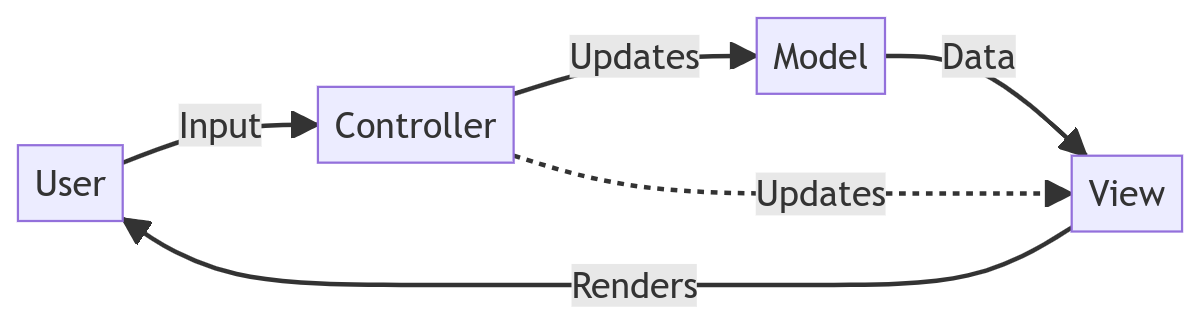
\includegraphics[width=\textwidth]{../images/mvc-classic.png}
	\caption{Classic MVC model when Users with controllers not screens}
	\label{fig:mvc-classic}
\end{figure}

\subsection{MVC dalam Kerangka Web dan Aplikasi Desktop Modern}

Banyak kerangka kerja web modern, seperti Laravel, Django, dan Spring, serta aplikasi desktop seperti JavaFX, menggunakan pendekatan MVC yang sedikit berbeda. Dalam implementasi ini:

\begin{itemize}
	\item Controller sering kali memiliki peran lebih besar, menangani logika bisnis dan interaksi dengan Model.
	\item View tidak hanya menampilkan data tetapi juga dapat berisi kode pemrograman untuk rendering dinamis.
	\item Model sering kali terintegrasi dengan ORM (\textit{Object-Relational Mapping}) untuk mempermudah akses ke basis data.
\end{itemize}

Diagram berikut menggambarkan perbedaan antara MVC klasik dan yang digunakan dalam kerangka kerja web dan aplikasi desktop modern:

\begin{figure}[h]
	\centering
	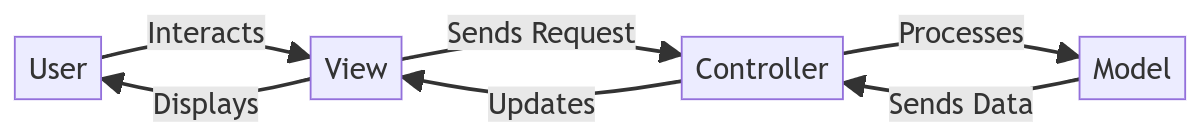
\includegraphics[width=\textwidth]{../images/mvc-modern.png}
	\caption{MVC in modern desktop/web frameworks.}
	\label{fig:mvc-modern}
\end{figure}

Pendekatan dalam kerangka kerja modern memungkinkan pemisahan lebih baik antara logika bisnis dan antarmuka pengguna, sekaligus mengintegrasikan teknologi seperti API REST dan AJAX untuk interaksi yang lebih dinamis.


\section{Model-View-Presenter (MVP)}

Model-View-Presenter (MVP) adalah pola desain yang mirip dengan MVC namun memiliki perbedaan signifikan dalam cara interaksi antara komponen-komponen tersebut. MVP lebih banyak digunakan dalam aplikasi desktop atau aplikasi yang membutuhkan pengendalian lebih besar terhadap tampilan dan interaksi pengguna. Dalam implementasi MVP:

\begin{itemize}
	\item \textbf{Model} bertanggung jawab untuk menangani logika bisnis dan data. Ini berinteraksi dengan basis data dan menyediakan data yang diperlukan oleh Presenter.
	\item \textbf{View} hanya bertugas untuk menampilkan antarmuka pengguna dan tidak mengandung logika bisnis. View akan menerima input dari pengguna dan meneruskannya ke Presenter. View bersifat pasif, artinya tidak mengelola pengolahan data atau logika bisnis.
	\item \textbf{Presenter} bertindak sebagai penghubung antara Model dan View. Presenter menerima input dari View, memprosesnya (dengan berinteraksi dengan Model), dan kemudian memperbarui View dengan data yang diperlukan.
\end{itemize}

Perbedaan utama antara \textbf{MVP} dan \textbf{MVC Klasik} terletak pada bagaimana komponen-komponen tersebut berinteraksi:
\begin{itemize}
	\item Dalam \textbf{MVP}, \textbf{Presenter} memiliki peran yang lebih besar. Semua logika bisnis dan pengolahan data dikelola oleh Presenter. View bertanggung jawab hanya untuk menampilkan data dan menerima input dari pengguna, tetapi tidak menangani pengolahan atau logika bisnis. Presenter mengelola interaksi antara Model dan View.
	\item Dalam \textbf{MVC Klasik}, \textbf{Controller} bertanggung jawab untuk menangani logika bisnis dan interaksi antara Model dan View. View hanya menampilkan data dan berinteraksi langsung dengan Controller. Dengan kata lain, Controller mempengaruhi tampilan berdasarkan aksi pengguna dengan mengubah Model, sedangkan View hanya berfungsi untuk menampilkan antarmuka pengguna.
	\item Dalam \textbf{MVP}, komunikasi antara View dan Presenter adalah dua arah, sementara dalam \textbf{MVC Klasik}, komunikasi lebih cenderung satu arah dari Controller ke View atau Model ke View.
\end{itemize}

Diagram berikut menggambarkan arsitektur MVP dan perbedaan utamanya dengan MVC Klasik:

\begin{figure}[h]
	\centering
	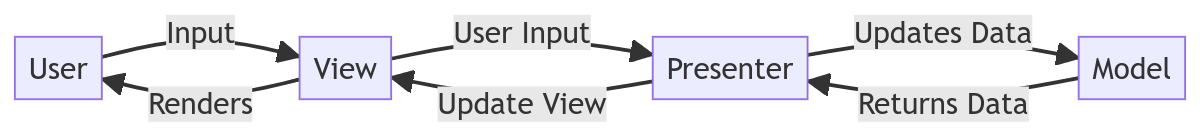
\includegraphics[width=\textwidth]{../images/mvp.png}
	\caption{Model-View-Presenter Architecture.}
	\label{fig:mvp-architecture}
\end{figure}

Keuntungan utama dari MVP adalah pemisahan yang jelas antara logika bisnis dan antarmuka pengguna, serta kemudahan pengujian unit karena Presenter dapat diuji secara terpisah tanpa bergantung pada View.

\section{Model-View-ViewModel (MVVM)}

Model-View-ViewModel (MVVM) adalah pola desain yang lebih banyak digunakan dalam aplikasi desktop dan aplikasi berbasis WPF (Windows Presentation Foundation) atau platform lain yang mendukung binding data dua arah. MVVM memisahkan logika presentasi dari antarmuka pengguna dengan cara yang sangat terstruktur. Dalam implementasi MVVM:

\begin{itemize}
	\item \textbf{Model} bertanggung jawab untuk menangani logika bisnis dan data. Model ini berinteraksi dengan basis data atau layanan lain untuk menyediakan data yang diperlukan oleh ViewModel.
	\item \textbf{View} bertanggung jawab untuk menampilkan antarmuka pengguna dan menerima input dari pengguna. View hanya berfokus pada rendering dan tidak mengelola logika atau data.
	\item \textbf{ViewModel} adalah penghubung antara View dan Model. ViewModel menangani logika presentasi, memanipulasi data yang diterima dari Model, dan menyediakan data tersebut dalam bentuk yang dapat digunakan oleh View. Dalam MVVM, ViewModel berinteraksi dengan View menggunakan binding data dua arah, yang memungkinkan pembaruan secara otomatis antara View dan ViewModel.
\end{itemize}

Perbedaan utama antara \textbf{MVVM} dan \textbf{MVP} terletak pada peran **ViewModel** dalam MVVM:
\begin{itemize}
	\item Dalam \textbf{MVVM}, \textbf{ViewModel} berfungsi untuk mempersiapkan data dari Model agar dapat digunakan oleh View. ViewModel mengelola logika presentasi dan menyediakan data dalam format yang dapat langsung dipakai oleh View.
	\item Dalam \textbf{MVP}, \textbf{Presenter} bertanggung jawab untuk memproses input dari View dan mengatur interaksi dengan Model, sementara View hanya menampilkan data dan tidak terlibat dalam pengolahan data atau logika.
	\item Dalam \textbf{MVVM}, komunikasi antara View dan ViewModel menggunakan binding data dua arah, memungkinkan pembaruan otomatis antara keduanya. Sebaliknya, dalam \textbf{MVP}, komunikasi antara View dan Presenter adalah satu arah, dimana Presenter memperbarui View dengan data yang diproses.
\end{itemize}

Diagram berikut menggambarkan arsitektur MVVM dan perbedaan utamanya dengan MVP:

\begin{figure}[h]
	\centering
	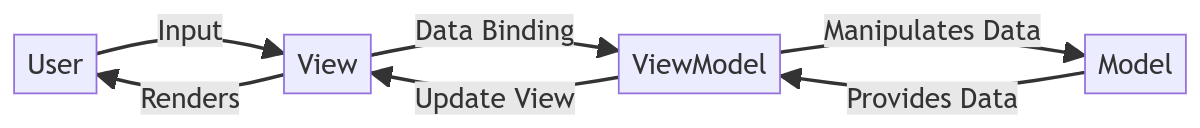
\includegraphics[width=\textwidth]{../images/mvvm.png}
	\caption{Model-View-ViewModel Architecture.}
	\label{fig:mvvm-architecture}
\end{figure}

Keuntungan utama dari MVVM adalah kemampuan untuk memisahkan logika presentasi dari antarmuka pengguna dengan menggunakan binding data dua arah, sehingga membuat pengujian dan pemeliharaan aplikasi lebih mudah. Selain itu, karena ViewModel menangani logika presentasi, View menjadi lebih sederhana dan lebih fokus pada rendering.


\section{Model-View-Intent (MVI)}

Model-View-Intent (MVI) adalah pola desain yang sering digunakan dalam aplikasi modern, terutama dalam pengembangan aplikasi Android. MVI bertujuan untuk menyederhanakan alur data dengan memberikan pendekatan yang lebih deklaratif dan reaktif. Dalam MVI, setiap komponen memiliki peran yang jelas dalam memanipulasi dan mengelola data aplikasi.

Dalam implementasi MVI:

\begin{itemize}
	\item \textbf{Model} berfungsi untuk menangani logika bisnis dan data aplikasi. Model ini menyediakan status atau keadaan aplikasi yang dapat digunakan oleh View. Model mengelola dan menyimpan data yang digunakan oleh aplikasi.
	\item \textbf{View} bertanggung jawab untuk menampilkan antarmuka pengguna dan menerima input dari pengguna. View akan mengirimkan intent ke Presenter atau ViewModel yang akan diproses lebih lanjut. View bersifat reaktif, menerima pembaruan dari Model melalui observasi data.
	\item \textbf{Intent} adalah tindakan atau niat yang dilakukan oleh pengguna yang kemudian diteruskan ke Presenter atau ViewModel untuk diproses. Intent menggambarkan apa yang ingin dilakukan oleh pengguna (misalnya, tombol ditekan atau elemen lainnya dipilih). Intent digunakan untuk memicu perubahan status pada Model atau memulai proses lain yang relevan.
\end{itemize}

Perbedaan utama antara \textbf{MVI} dan \textbf{MVP} terletak pada cara interaksi dan komunikasi antar komponen:
\begin{itemize}
	\item Dalam \textbf{MVI}, \textbf{Intent} menggantikan peran input pengguna yang secara langsung diteruskan ke ViewModel atau Presenter. Intent memfokuskan pada pengelolaan status aplikasi secara reaktif.
	\item Dalam \textbf{MVP}, \textbf{Presenter} bertanggung jawab untuk menangani logika presentasi dan memproses input dari View untuk memperbarui Model.
	\item Dalam \textbf{MVI}, komunikasi adalah satu arah dari Intent ke ViewModel atau Presenter, yang kemudian memodifikasi status Model dan mengirimkan pembaruan kembali ke View.
\end{itemize}

Diagram berikut menggambarkan arsitektur MVI dan perbedaannya dengan pola desain lain seperti MVP:

\begin{figure}[h]
	\centering
	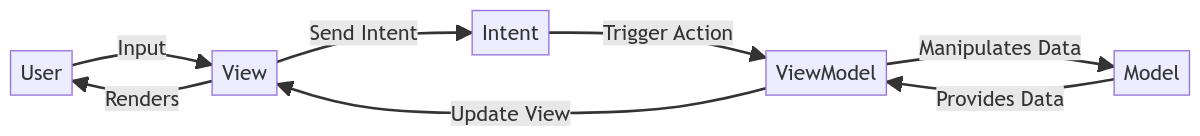
\includegraphics[width=\textwidth]{../images/mvi.png}
	\caption{Model-View-Intent Architecture.}
	\label{fig:mvi-architecture}
\end{figure}

Keuntungan utama dari MVI adalah pengelolaan status aplikasi yang lebih sederhana dan kemampuan untuk menangani alur data yang lebih reaktif. MVI juga memudahkan pemeliharaan kode dengan mengurangi kebingungan terkait interaksi antara View dan Model, serta memperkenalkan pendekatan yang lebih terstruktur untuk menangani state.


\section{Contoh:}

Bagian ini menyajikan contoh implementasi arsitektur perangkat lunak menggunakan bahasa pemrograman Java dengan pustaka Java Swing. Implementasi ini menggunakan dua buah komponen \texttt{JSpinner}, di mana perubahan nilai pada \texttt{JSpinner} asal akan mempengaruhi nilai pada \texttt{JSpinner} tujuan. Perubahan nilai tidak terjadi secara langsung, melainkan diproses terlebih dahulu sesuai dengan arsitektur yang digunakan.

Setiap arsitektur memiliki pendekatan yang berbeda dalam menangani perubahan nilai pada \texttt{JSpinner}. Dalam Model-View-Controller (MVC), perubahan nilai dikelola oleh controller, yang bertanggung jawab sebagai perantara antara tampilan dan model. Dalam Model-View-Presenter (MVP), presenter mengambil alih peran perantara dengan mengelola logika pembaruan nilai. Model-View-ViewModel (MVVM) menggunakan mekanisme binding untuk menyinkronkan perubahan nilai antara tampilan dan model secara otomatis. Sementara itu, Model-View-Intent (MVI) menggunakan intent sebagai mekanisme untuk mengirimkan perubahan dari tampilan ke model.

Setiap arsitektur yang disajikan dalam bagian ini akan disertai dengan diagram urutan (sequence diagram) untuk menjelaskan bagaimana interaksi antara komponen terjadi dalam menangani perubahan nilai pada \texttt{JSpinner}. Diagram tersebut akan memberikan gambaran bagaimana data mengalir dari tampilan ke model serta bagaimana nilai diperbarui dalam sistem.


\subsection{Model-View-Controller (MVC)}
\begin{figure}[h]
	\centering
	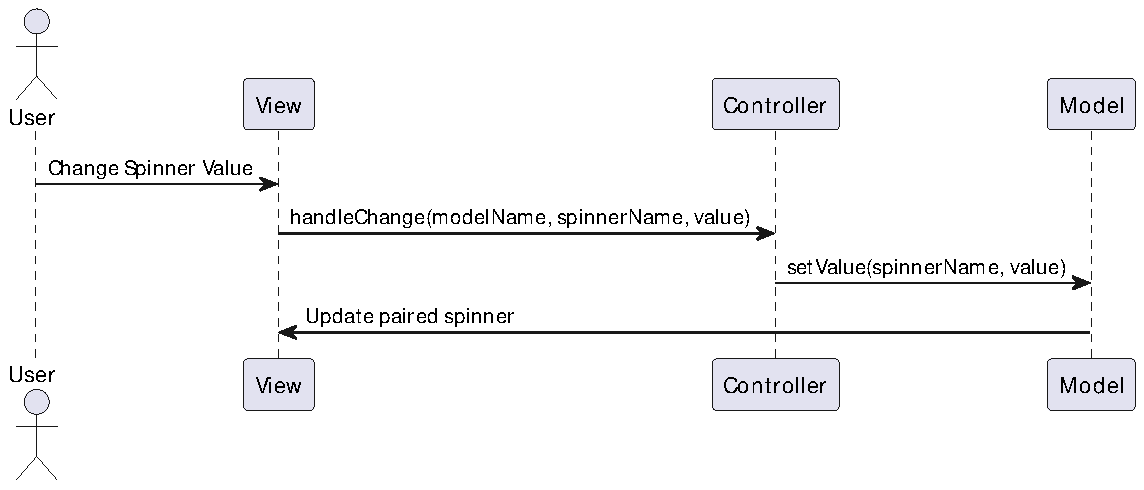
\includegraphics[width=\textwidth]{../images/out/mvc-sequence}
	\caption{Model-View-Sequence Architecture.}
	\label{fig:mvc-sequence}
\end{figure}

Diagram urutan ini menggambarkan interaksi antara pengguna, tampilan (view), controller, dan model dalam arsitektur Model-View-Controller (MVC). Diagram ini menjelaskan bagaimana perubahan dalam antarmuka pengguna diproses melalui controller sebelum diperbarui di model dan tampilan.

Ketika \textbf{Pengguna} mengubah nilai pada spinner di antarmuka grafis, aksi ini ditangkap oleh \textbf{View}. Selanjutnya, view meneruskan perubahan ini ke \textbf{Controller} melalui metode \texttt{handleChange()} dengan parameter nama model, nama spinner, dan nilai baru.

Controller bertindak sebagai perantara antara view dan model dengan langkah-langkah sebagai berikut:

\begin{itemize}
	\item Controller menerima permintaan perubahan dari view dan meneruskannya ke \textbf{Model} dengan memanggil metode \texttt{setValue()} untuk memperbarui data yang sesuai.
	\item Model kemudian memperbarui data internalnya dengan nilai baru yang diberikan oleh controller.
	\item Setelah perubahan data selesai, model memperbarui \textbf{View} agar tampilan merefleksikan perubahan nilai yang telah terjadi.
\end{itemize}

Dalam arsitektur MVC, \textbf{Controller} bertanggung jawab untuk menangani interaksi pengguna dan meneruskan data ke model. Model menyimpan dan mengelola logika bisnis serta perubahan data, sementara view hanya menampilkan hasil tanpa menangani logika bisnis secara langsung.

Pendekatan ini memisahkan logika aplikasi dari antarmuka pengguna, membuat kode lebih mudah dipelihara dan diperluas. Selain itu, arsitektur MVC memungkinkan modularitas yang lebih besar, di mana model dan view dapat diperbarui atau diganti tanpa mengubah komponen lainnya.

Secara keseluruhan, diagram urutan ini menunjukkan bagaimana Model-View-Controller (MVC) mengelola aliran data dengan pendekatan yang lebih terstruktur, memastikan keterpisahan yang jelas antara presentasi, logika bisnis, dan data.


\subsection{Model-View-Presenter (MVP)}
\begin{figure}[h]
	\centering
	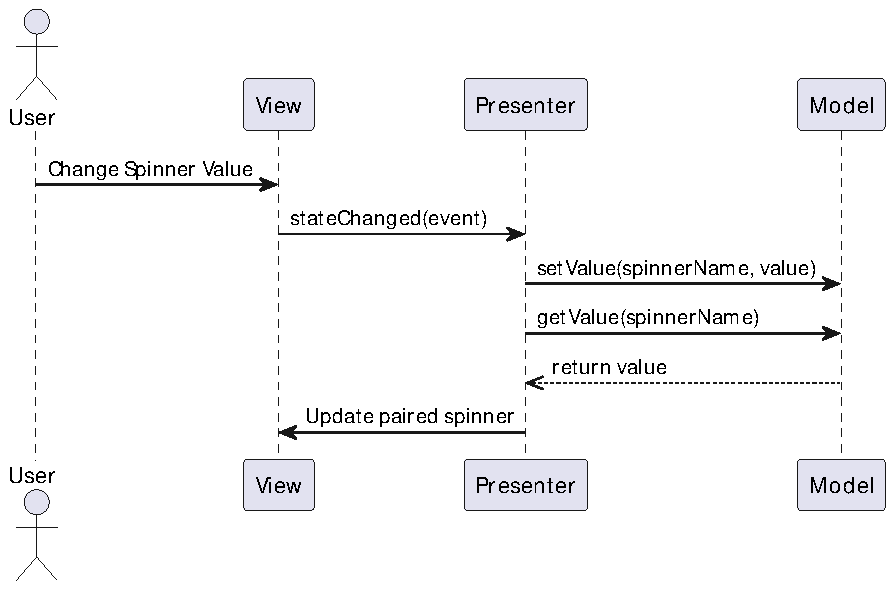
\includegraphics[width=\textwidth]{../images/out/mvp-sequence}
	\caption{Model-View-Presenter Sequence Architecture.}
	\label{fig:mvp-sequence}
\end{figure}

Diagram urutan ini menggambarkan interaksi antara pengguna, tampilan (view), presenter, dan model dalam arsitektur Model-View-Presenter (MVP). Diagram ini menjelaskan bagaimana perubahan dalam antarmuka pengguna diproses dan dikendalikan oleh presenter sebelum diperbarui di model dan tampilan.

Ketika \textbf{Pengguna} mengubah nilai pada spinner di antarmuka grafis, aksi ini ditangkap oleh \textbf{View}. Selanjutnya, view meneruskan perubahan ini ke \textbf{Presenter} melalui metode \texttt{stateChanged()}.

Presenter bertindak sebagai perantara antara view dan model dengan langkah-langkah sebagai berikut:

\begin{itemize}
	\item Presenter mengirimkan nilai baru ke \textbf{Model} dengan memanggil metode \texttt{setValue()} untuk memperbarui data yang sesuai.
	\item Setelah nilai diperbarui, presenter mengambil kembali nilai terbaru dari model dengan memanggil metode \texttt{getValue()}.
	\item Model mengembalikan nilai yang diperbarui ke presenter.
	\item Presenter kemudian memperbarui tampilan dengan mengirimkan nilai terbaru ke \textbf{View}, memastikan bahwa antarmuka pengguna mencerminkan perubahan yang telah terjadi.
\end{itemize}

Dalam arsitektur MVP, \textbf{Presenter} bertanggung jawab penuh untuk menangani logika aplikasi dan komunikasi antara view serta model. Hal ini memastikan bahwa view hanya menangani rendering antarmuka pengguna tanpa menyimpan atau mengelola data bisnis.

Pendekatan ini meningkatkan pemisahan tanggung jawab (Separation of Concerns), membuat kode lebih mudah diuji karena presenter dapat diuji secara terpisah dari view. Selain itu, arsitektur MVP memungkinkan fleksibilitas yang lebih besar dalam mengganti tampilan tanpa mengubah logika aplikasi di presenter.

Secara keseluruhan, diagram urutan ini menunjukkan bagaimana Model-View-Presenter (MVP) mengelola aliran data dan pembaruan tampilan dengan pendekatan yang lebih terstruktur dan terorganisir.


\subsection{Model-View-ViewModel (MVVM)}
\begin{figure}[h]
	\centering
	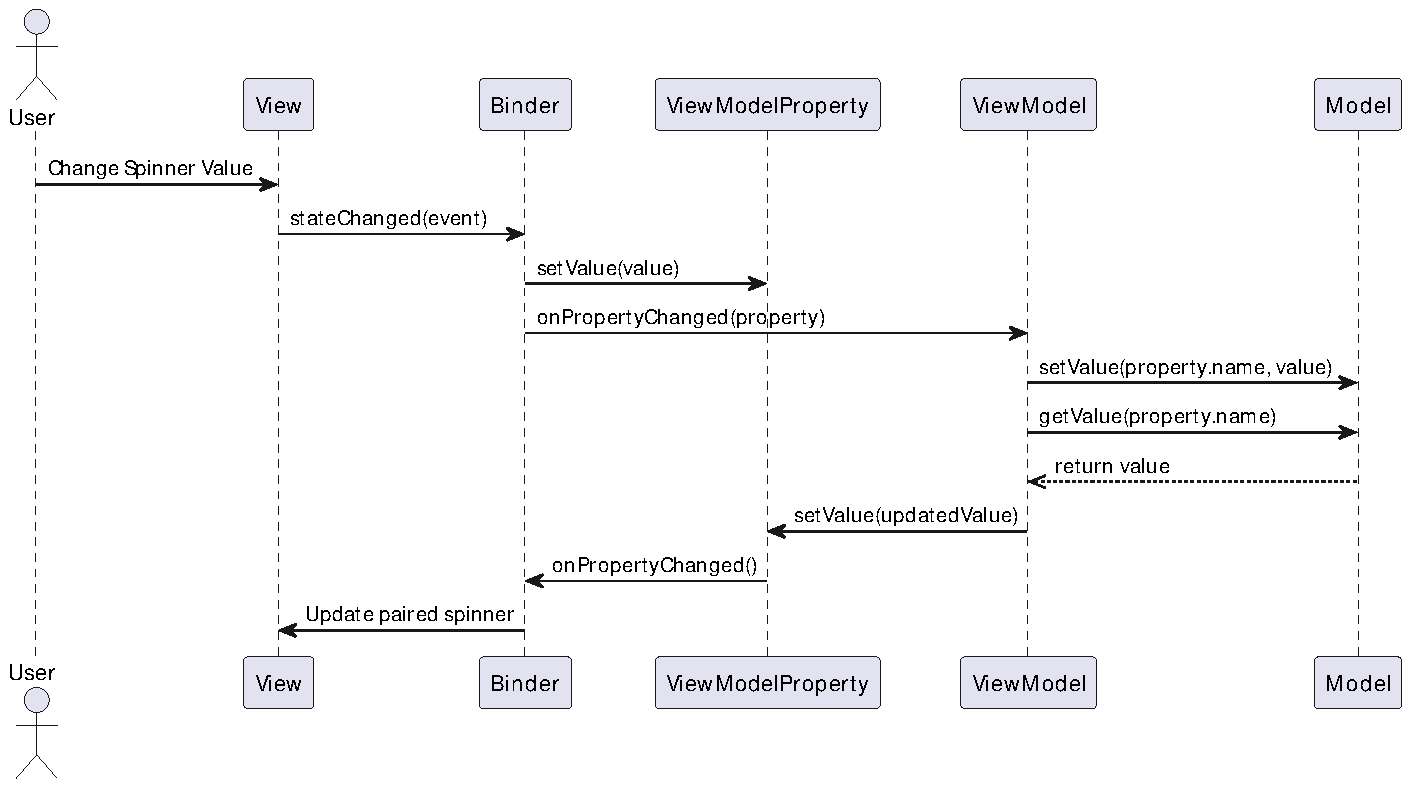
\includegraphics[width=\textwidth]{../images/out/mvvm-sequence}
	\caption{Model-View-ViewModel Sequence Architecture.}
	\label{fig:mvvm-sequence}
\end{figure}

Diagram urutan ini menggambarkan interaksi antara pengguna, tampilan (view), binder, properti ViewModel, ViewModel, dan model dalam arsitektur Model-View-ViewModel (MVVM). Diagram ini menjelaskan bagaimana perubahan dalam antarmuka pengguna diproses dan disinkronkan dengan model menggunakan mekanisme binding.

Ketika \textbf{Pengguna} mengubah nilai pada spinner di antarmuka grafis, aksi ini ditangkap oleh \textbf{View}. Selanjutnya, view mengirimkan perubahan ini ke \textbf{Binder} melalui metode \texttt{stateChanged()}. Binder bertugas untuk menjembatani komunikasi antara ViewModelProperty dan ViewModel.

Binder kemudian melakukan langkah-langkah berikut untuk memastikan data tetap sinkron antara view dan model:

\begin{itemize}
	\item Binder mengubah nilai pada \textbf{ViewModelProperty} dengan memanggil metode \texttt{setValue()}.
	\item Setelah nilai diperbarui, binder memberi tahu \textbf{ViewModel} tentang perubahan ini melalui metode \texttt{onPropertyChanged()}.
	\item ViewModel kemudian memperbarui \textbf{Model} dengan memanggil metode \texttt{setValue()} untuk menyimpan nilai baru.
	\item Setelah itu, ViewModel mengambil nilai terbaru dari Model menggunakan metode \texttt{getValue()}.
	\item Model mengembalikan nilai yang diperbarui ke ViewModel.
	\item ViewModel memperbarui nilai dalam \textbf{ViewModelProperty} dengan nilai yang baru.
	\item ViewModelProperty memberi tahu \textbf{Binder} bahwa perubahan telah terjadi melalui metode \texttt{onPropertyChanged()}.
	\item Terakhir, binder memperbarui tampilan (View) agar komponen yang terkait mencerminkan nilai yang telah diperbarui.
\end{itemize}

Arsitektur MVVM memastikan bahwa tampilan hanya berfungsi sebagai antarmuka pengguna tanpa menangani logika bisnis secara langsung. Binder bertugas sebagai penghubung antara View dan ViewModel untuk memastikan sinkronisasi data berjalan otomatis. 

Dengan menggunakan properti ViewModel dan mekanisme binding, arsitektur ini memungkinkan pemisahan tanggung jawab yang lebih jelas antara lapisan presentasi dan data. Pendekatan ini meningkatkan pemeliharaan kode dan memungkinkan pengujian yang lebih mudah karena ViewModel dapat diuji secara terpisah dari tampilan.

Secara keseluruhan, diagram urutan ini menunjukkan bagaimana Model-View-ViewModel (MVVM) mengelola perubahan status dengan cara yang terorganisir dan efisien, memastikan bahwa data selalu tersinkronisasi antara model dan tampilan.


\subsection{Model-View-Intent (MVI)}
\begin{figure}[h]
	\centering
	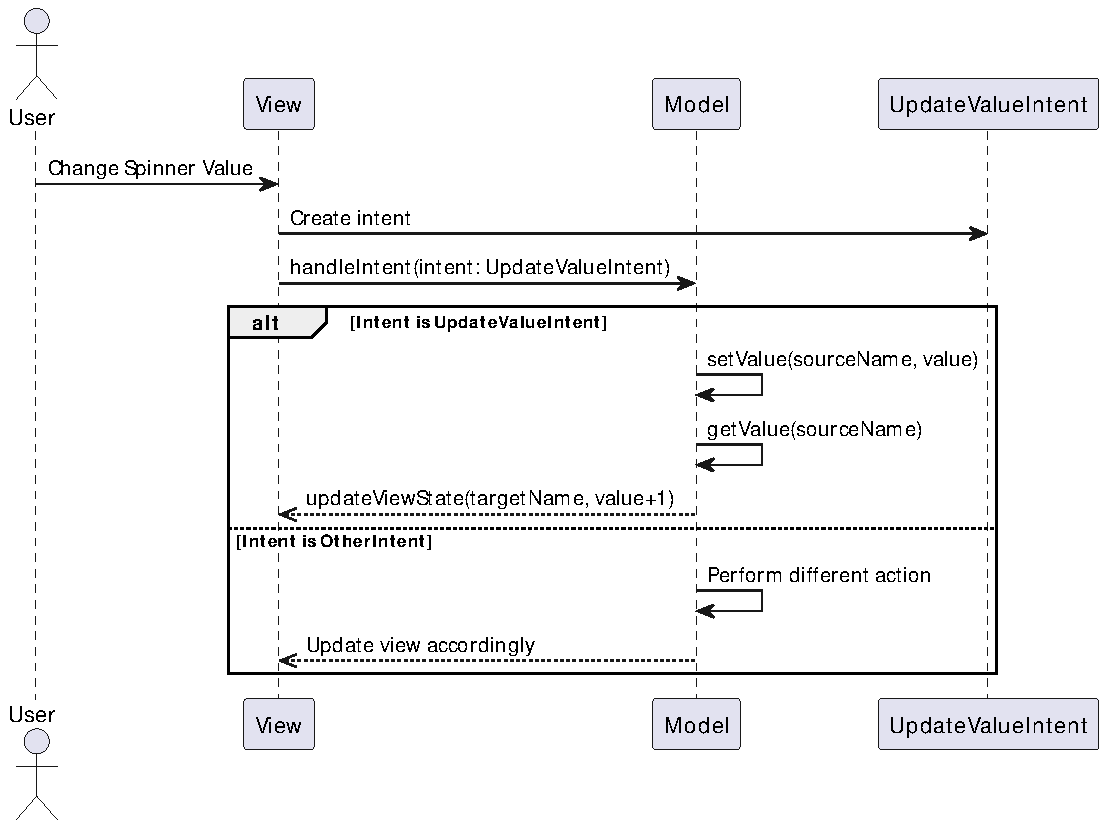
\includegraphics[width=\textwidth]{../images/out/mvi-sequence}
	\caption{Model-View-Intent Sequence Architecture.}
	\label{fig:mvi-sequence}
\end{figure}

Diagram urutan ini menggambarkan interaksi antara pengguna, tampilan (view), model, dan intent dalam arsitektur Model-View-Intent (MVI). Diagram ini menjelaskan bagaimana perubahan dalam antarmuka pengguna diproses dan diteruskan melalui sistem.

Ketika \textbf{Pengguna} mengubah nilai pada spinner di antarmuka grafis, aksi ini ditangkap oleh \textbf{View}. Selanjutnya, view membuat sebuah instance dari \texttt{UpdateValueIntent}, yang berisi nilai baru yang akan diperbarui serta komponen target yang akan menerima nilai tersebut. Intent ini berfungsi sebagai pesan terstruktur yang memberikan instruksi kepada model mengenai perubahan yang perlu dilakukan.

Setelah intent dibuat, view memanggil metode \texttt{handleIntent()} pada \textbf{Model}, dengan mengirimkan \texttt{UpdateValueIntent} sebagai parameter. Model kemudian memproses intent berdasarkan tipenya dengan mekanisme percabangan sebagai berikut:

\begin{itemize}
	\item \textbf{Jika intent adalah \texttt{UpdateValueIntent}}, model akan memperbarui nilai yang sesuai dengan memanggil metode \texttt{setValue()}. Selanjutnya, nilai yang diperbarui diambil kembali menggunakan metode \texttt{getValue()}. Setelah itu, model akan memperbarui tampilan dengan memanggil metode \texttt{updateViewState()} dan mengirimkan nilai yang telah diperbarui. Hal ini memastikan bahwa antarmuka pengguna selalu merefleksikan perubahan yang terjadi di dalam model.
	\item \textbf{Jika intent adalah tipe lain (\texttt{OtherIntent})}, model akan menjalankan aksi berbeda, yang mungkin melibatkan perhitungan tambahan atau perubahan status lainnya. Setelah operasi yang sesuai dijalankan, model akan memperbarui tampilan agar perubahan yang terjadi dapat terlihat pada antarmuka pengguna.
\end{itemize}

Arsitektur ini memastikan pemisahan tanggung jawab yang jelas dengan mendelegasikan pembaruan UI ke view, sementara model bertanggung jawab atas logika bisnis dan pengelolaan data. Pola ini meningkatkan kemudahan pemeliharaan serta pengujian dengan mengurangi keterkaitan langsung antara antarmuka pengguna dan logika aplikasi.

Dengan menggunakan intent, sistem menyediakan mekanisme terstruktur untuk mengelola perubahan status antara view dan model. Pendekatan ini memungkinkan manajemen status yang lebih baik dan memastikan bahwa semua perubahan diproses secara eksplisit melalui model, bukan langsung dimodifikasi di dalam view.

Secara keseluruhan, diagram urutan ini merepresentasikan implementasi arsitektur Model-View-Intent yang kuat, yang mendorong aliran data searah dan mengurangi ketergantungan antara komponen.
